\documentclass[twoside,11pt]{article}
\usepackage[preprint,abbrvbib]{jmlr2e}
\usepackage[T1]{fontenc}
\usepackage{lmodern}
\usepackage{amsmath}
\usepackage{booktabs}
\usepackage{multirow}
\usepackage{float}
% generated by code/make_tables.py; do not edit
\newcommand{\nItems}{5{,}421}
\newcommand{\nModels}{37}
\newcommand{\nLabelErrA}{100}
\newcommand{\errRateA}{1.84}
\newcommand{\hiddenMinA}{8}
\newcommand{\hiddenMaxA}{30}
\newcommand{\hiddenMedA}{17}
\newcommand{\inflMinA}{0.15}
\newcommand{\inflMaxA}{0.55}
\newcommand{\rankGainA}{3}
\newcommand{\favFlaggersA}{7}
\newcommand{\indepRatioA}{1.8}
\newcommand{\allPanelAdjA}{5{,}051}
\newcommand{\topTenHiddenA}{7}
\newcommand{\topTenAdjA}{2{,}164}
\newcommand{\allPanelAdjPctA}{93}
\newcommand{\hiddenTopFiveMinA}{16}
\newcommand{\hiddenTopFiveMaxA}{20}
\newcommand{\adjTopFiveMinA}{802}
\newcommand{\adjTopFiveMaxA}{1045}
\newcommand{\errRateBmin}{21.0}
\newcommand{\errRateBmax}{29.6}
\newcommand{\inflMinB}{4.9}
\newcommand{\inflMaxB}{13.9}
\newcommand{\favFlaggersBmin}{32}
\newcommand{\favFlaggersBmax}{33}
\newcommand{\rankGainBmin}{13}
\newcommand{\rankGainBmax}{27}
\newcommand{\indepRatioBmin}{4.3}
\newcommand{\indepRatioBmax}{4.9}
\newcommand{\llamaInflB}{9.7}
\newcommand{\llamaTrueRankB}{6}
\newcommand{\llamaDrRankB}{1}
\newcommand{\llamaFavB}{5}
\newcommand{\errRateBmain}{26.5}
\newcommand{\drFlagRmseA}{0.35}
\newcommand{\tpWaldCovOneA}{0.14}
\newcommand{\tpWaldCovTwentyA}{0.90}
\newcommand{\tpCpCovMinA}{0.997}
\newcommand{\tpMaxBiasA}{0.04}
\newcommand{\tpFlagRmseTenA}{0.25}
\newcommand{\tpAdjTenA}{1279}
\newcommand{\tpAdjDRA}{819}
\newcommand{\drFlagRmseB}{9.72}
\newcommand{\tpWaldCovOneB}{0.93}
\newcommand{\tpWaldCovTwentyB}{0.95}
\newcommand{\tpCpCovMinB}{0.988}
\newcommand{\tpMaxBiasB}{0.25}
\newcommand{\tpFlagRmseTenB}{1.29}
\newcommand{\tpAdjTenB}{1595}
\newcommand{\tpAdjDRB}{1170}
\newcommand{\reps}{2{,}000}
\newcommand{\hiddenGptA}{19}
\newcommand{\allocUnifOneA}{0.38}
\newcommand{\allocNeyOneA}{0.27}
\newcommand{\allocNeyPiDOneA}{0.46}
\newcommand{\eDA}{0.076}
\newcommand{\eCA}{0.0032}
\newcommand{\nDA}{819}
\newcommand{\nCA}{4602}
\newcommand{\allocUnifOneB}{1.16}
\newcommand{\allocNeyOneB}{1.03}
\newcommand{\allocNeyPiDOneB}{0.40}
\newcommand{\eDB}{0.575}
\newcommand{\eCB}{0.0976}
\newcommand{\nDB}{1170}
\newcommand{\nCB}{4251}
\newcommand{\lockGptOneB}{3.4}
\newcommand{\lockOpusOneB}{3.4}
\newcommand{\lockHiddenOneB}{676}
\newcommand{\lockHiddenLastB}{142}
\newcommand{\lockAdjOneB}{1333}
\newcommand{\lockAdjLastB}{2644}
\newcommand{\lockPanelLastB}{5}
\newcommand{\lockGptCorrectOneB}{391}
\newcommand{\lockGptRepeatOneB}{208}
\newcommand{\lockGptCorrectPpOneB}{7.2}
\newcommand{\lockGptRepeatPpOneB}{3.8}
\newcommand{\lockOpusCorrectOneB}{388}
\newcommand{\lockOpusRepeatOneB}{205}
\newcommand{\lockHiddenLastA}{4}
\newcommand{\lockAdjLastA}{2817}
\newcommand{\sensTrueRateA}{0.0041}
\newcommand{\sensPairTrueA}{0.35}
\newcommand{\sensPairDRA}{0.20}
\newcommand{\sensPairDRAabs}{0.20}
\newcommand{\sensEpsCoverA}{0.001}
\newcommand{\sensEpsSignA}{0}
\newcommand{\sensTrueRateB}{0.1240}
\newcommand{\sensPairTrueB}{0.57}
\newcommand{\sensPairDRB}{-8.65}
\newcommand{\sensPairDRBabs}{8.65}
\newcommand{\sensEpsCoverB}{0.075}
\newcommand{\sensEpsSignB}{0.075}
\newcommand{\rateEps}{0.124}
\newcommand{\rateGamma}{0.784}
\newcommand{\rateRatioMin}{0.98}
\newcommand{\rateRatioMax}{1.03}
\newcommand{\nOk}{5{,}321}
\newcommand{\nWrongGt}{100}
\newcommand{\nBadQ}{131}
\newcommand{\nMulti}{38}
\newcommand{\nNoCorrect}{36}
\newcommand{\nExpert}{32}
\newcommand{\nBadOpt}{25}
\newcommand{\nNoMatch}{10}
\newcommand{\nUnparsed}{5}
\newcommand{\nSameAsLabel}{1}
\newcommand{\nLabelDiffers}{1}
\newcommand{\helmDisagreeTotal}{29}
\newcommand{\helmDisagreeMax}{3}
\newcommand{\helmInstances}{14{,}042}
\newcommand{\invalidMax}{994}
\newcommand{\invalidMaxModel}{Mistral Large}
\newcommand{\invalidZero}{22}
\newcommand{\simCovMinA}{0.962}
\newcommand{\simWidthOneA}{11.7}
\newcommand{\simWidthFiveA}{3.2}
\newcommand{\simWidthHalfA}{0.7}
\newcommand{\simPairWidthFiveA}{6.1}
\newcommand{\simPairWidthHalfA}{1.3}
\newcommand{\simCertFiveA}{11}
\newcommand{\simCertHalfA}{50}
\newcommand{\simNoErrOneA}{84}
\newcommand{\simTrueCertA}{97}
\newcommand{\simNadjA}{36}
\newcommand{\cpWidthOneA}{16.2}
\newcommand{\waldPairCovOneA}{0.03--0.06}
\newcommand{\simCovMinB}{0.953}
\newcommand{\simWidthOneB}{29.5}
\newcommand{\simWidthFiveB}{22.0}
\newcommand{\simWidthHalfB}{10.2}
\newcommand{\simPairWidthFiveB}{26.0}
\newcommand{\simPairWidthHalfB}{13.3}
\newcommand{\simCertFiveB}{0}
\newcommand{\simCertHalfB}{3}
\newcommand{\simNoErrOneB}{0}
\newcommand{\simTrueCertB}{97}
\newcommand{\simNadjB}{35}
\newcommand{\cpWidthOneB}{26.5}
\newcommand{\waldPairCovOneB}{0.82--0.89}
\newcommand{\simWrongMax}{0}
\newcommand{\cnItems}{46{,}328}
\newcommand{\cnExcluded}{107}
\newcommand{\cnAdj}{1{,}393}
\newcommand{\cnAdjPct}{3.0}
\newcommand{\cnFlagged}{1{,}230}
\newcommand{\cnIncidental}{163}
\newcommand{\cnRefErr}{287}
\newcommand{\cnRefErrIn}{179}
\newcommand{\cnHidden}{108}
\newcommand{\cnHiddenPct}{38}
\newcommand{\cnReissChanges}{475}
\newcommand{\cnAgreeChanges}{149}
\newcommand{\cnDisagreeIn}{347}
\newcommand{\cnTau}{0.988}
\newcommand{\cnNinv}{1}
\newcommand{\cnNmodels}{21}
\newcommand{\cnHiddenAbsMax}{0.14}
\newcommand{\cnHiddenMin}{-0.02}
\newcommand{\cnHiddenMax}{+0.14}
\newcommand{\cnAdjMin}{-0.41}
\newcommand{\cnAdjMax}{-0.28}
\newcommand{\cnAllHiddenPos}{not every}
\newcommand{\cnConcRate}{0.24}
\newcommand{\cnHiddenEntrantMean}{+0.064}
\newcommand{\cnHiddenHfMean}{+0.030}
\newcommand{\cnNhf}{5}
\newcommand{\cnNentrant}{16}
\newcommand{\cnInvA}{Carreras (b) (2003)}
\newcommand{\cnInvB}{McCallum (2003)}
\newcommand{\cnInvGap}{0.03}
\newcommand{\cnPairA}{Florian (2003)}
\newcommand{\cnPairB}{Chieu (2003)}
\newcommand{\cnPairDR}{0.011}
\newcommand{\cnPairTrue}{0.188}
\newcommand{\cnPairEpsAmbig}{0.0005}
\newcommand{\cnWidthTwo}{0.39}
\newcommand{\cnEnt}{8{,}169}
\newcommand{\cnEntHiddenMin}{-0.10}
\newcommand{\cnEntHiddenMax}{+0.78}
\newcommand{\cnEntAdjMin}{-2.47}
\newcommand{\cnEntAdjMax}{-1.70}
\newcommand{\cnEntTau}{0.990}
\newcommand{\cnEntNinv}{1}
\newcommand{\cnEntInvA}{Hendrickx (2003)}
\newcommand{\cnEntInvB}{Wu (2003)}
\newcommand{\cnEntInvGap}{0.06}
\newcommand{\cnTies}{1}
\newcommand{\cnPairs}{210}
\newcommand{\cnDisagreeChanges}{326}
\newcommand{\sweepN}{37}
\newcommand{\sweepErrMin}{13.9}
\newcommand{\sweepErrMax}{70.6}
\newcommand{\sweepBestLabeler}{Claude 3 Opus}
\newcommand{\sweepBestErr}{13.9}
\newcommand{\sweepBestMedInfl}{6.1}
\newcommand{\sweepBestMaxGain}{8}
\newcommand{\sweepMedInflMin}{6.1}
\newcommand{\sweepMedInflMax}{10.9}
\newcommand{\sweepMaxGainMax}{32}
\newcommand{\sweepFavMin}{31}
\newcommand{\dupAgree}{99.85}
\newcommand{\dupDiffer}{8}

\renewcommand{\thetable}{OA.\arabic{table}}
\renewcommand{\thefigure}{OA.\arabic{figure}}
\usepackage{graphicx}
\newcommand{\Dset}{\Delta}
\ShortHeadings{Discrepant Resolution in Benchmark Relabelling: Online Appendix}{}
\firstpageno{1}
\begin{document}
\title{Online Appendix to ``Only Checking Where the Model Disagrees:\\ Discrepant-Resolution Bias in Benchmark Relabelling''}
\maketitle

This online appendix describes the data processing and the literature-coding protocol, and gives two tables and a figure that support Section~7 of the paper. Code and data are at \url{https://github.com/unluckyjet/discrepant-resolution}.

\section{Data processing (MMLU-Redux and HELM)}


MMLU-Redux 2.0 contains 5{,}700 items. The analysis set has \nItems{} items: the \nOk{} items annotated as correct and the \nWrongGt{} items annotated with a wrong ground truth and a parseable corrected answer. We exclude the following items:
\begin{itemize}
\item \nBadQ{} with bad question clarity;
\item \nMulti{} with multiple correct answers;
\item \nNoCorrect{} with no correct answer;
\item \nExpert{} marked ``expert'';
\item \nBadOpt{} with bad option clarity;
\item \nUnparsed{} marked as wrong ground truth whose suggested answer could not be parsed;
\item \nSameAsLabel{} marked as wrong ground truth whose suggested answer equals the MMLU label;
\item \nNoMatch{} that could not be matched to a HELM instance;
\item \nLabelDiffers{} whose MMLU-Redux copy of the label differs from HELM's.
\end{itemize}
The suggested answer appears in several formats (an index, a float, a letter); a parser handles all of them.

We downloaded HELM v1.3.0 per-instance predictions for all \nModels{} models and 57 subjects (\helmInstances{} instances per model; method \texttt{multiple\_choice\_joint}). A prediction is parsed as an option letter only if the output begins with a bare letter A--D, optionally in parentheses and not followed by another letter. Every other output is invalid and counts as wrong under every label. Our parsed correctness agrees with HELM's exact-match scores on all but \helmDisagreeTotal{} of the $\nModels\times\helmInstances$ instance predictions (at most \helmDisagreeMax{} per model). The disagreements are items with duplicated option texts, which HELM scores by text.

Invalid outputs in the analysis set range from zero (for \invalidZero{} models) to \invalidMax{} (\invalidMaxModel). In Scenario B an invalid labeler output becomes a deliberately wrong label. All scripts, the derived item-level table and the results files are released.

\section{Literature coding protocol}


Candidate studies were collected from Semantic Scholar searches for benchmark relabelling, label-error audits and benchmark cleaning, and from the reference lists of the studies found. For each study we read the methods section in full text. We then recorded the following:
\begin{itemize}
\item the adjudication design, in the categories of Section~6 of the paper;
\item the flagging model or algorithm;
\item whether a flagging model was also evaluated on the corrected labels;
\item whether accuracies or rankings were re-reported;
\item whether the paper acknowledges that unflagged items may be mislabelled.
\end{itemize}
Each code is supported by a verbatim quote with its page. A script checks every quote against the extracted full text, and all quotes matched. Confidence was recorded as high or medium; no study was coded without a supporting quote. Studies whose phases follow different designs are coded OTHER. The coding table, with quotes, is released as \texttt{data/lit/design\_coding.csv}.


\section{Additional tables}

\begin{table}[H]
\centering
\scriptsize
\begin{tabular}{lrrrrrrr}
\toprule
Flagger & True acc.\ (\%) & Adjudicated & Hidden $|J|$ & Inflation (pp) & True rank & DR rank & Flagger-favouring \\
\midrule
Claude 3 Opus & 86.13 & 802 & 17 & 0.31 & 1 & 1 & 0 \\
GPT-4o & 85.78 & 819 & 19 & 0.35 & 2 & 2 & 0 \\
GPT-4 (0613) & 84.63 & 879 & 17 & 0.31 & 3 & 3 & 0 \\
Gemini 1.5 Pro & 82.92 & 973 & 20 & 0.37 & 4 & 4 & 0 \\
GPT-4 Turbo & 81.55 & 1045 & 16 & 0.30 & 5 & 5 & 0 \\
Llama 3 70B & 80.98 & 1075 & 19 & 0.35 & 6 & 6 & 0 \\
PaLM 2 Unicorn & 80.39 & 1109 & 19 & 0.35 & 7 & 7 & 0 \\
Palmyra X v3 & 80.37 & 1110 & 19 & 0.35 & 8 & 8 & 0 \\
Mixtral 8x22B & 79.60 & 1147 & 22 & 0.41 & 9 & 9 & 0 \\
Gemini 1.5 Flash & 79.54 & 1148 & 20 & 0.37 & 10 & 9 & 1 \\
Qwen1.5 72B & 79.04 & 1182 & 16 & 0.30 & 11 & 11 & 0 \\
Claude 3 Sonnet & 77.81 & 1245 & 22 & 0.41 & 12 & 12 & 0 \\
Yi 34B & 77.64 & 1255 & 18 & 0.33 & 13 & 13 & 0 \\
Qwen1.5 32B & 76.00 & 1342 & 20 & 0.37 & 14 & 14 & 0 \\
Claude 3 Haiku & 75.74 & 1359 & 18 & 0.33 & 15 & 15 & 0 \\
DBRX Instruct & 75.61 & 1364 & 17 & 0.31 & 16 & 15 & 1 \\
Claude 2.1 & 75.36 & 1383 & 19 & 0.35 & 17 & 16 & 1 \\
DeepSeek 67B & 73.88 & 1456 & 19 & 0.35 & 18 & 18 & 0 \\
Mixtral 8x7B & 73.53 & 1486 & 14 & 0.26 & 19 & 19 & 0 \\
Gemini 1.0 Pro & 71.87 & 1583 & 8 & 0.15 & 20 & 20 & 0 \\
Llama 2 70B & 71.15 & 1610 & 14 & 0.26 & 21 & 21 & 0 \\
Mistral Large & 70.98 & 1609 & 13 & 0.24 & 22 & 22 & 0 \\
PaLM 2 Bison & 70.93 & 1624 & 14 & 0.26 & 23 & 22 & 1 \\
Mistral Small & 70.93 & 1622 & 11 & 0.20 & 23 & 22 & 1 \\
Qwen1.5 14B & 70.84 & 1635 & 13 & 0.24 & 25 & 22 & 2 \\
Claude Instant 1.2 & 70.65 & 1637 & 15 & 0.28 & 26 & 25 & 1 \\
GPT-3.5 Turbo & 70.39 & 1646 & 17 & 0.31 & 27 & 27 & 0 \\
Arctic Instruct & 69.06 & 1719 & 19 & 0.35 & 28 & 28 & 0 \\
Llama 3 8B & 68.86 & 1735 & 15 & 0.28 & 29 & 29 & 0 \\
Gemma 7B & 67.42 & 1807 & 17 & 0.31 & 30 & 30 & 0 \\
Yi 6B & 65.49 & 1910 & 16 & 0.30 & 31 & 31 & 0 \\
Qwen1.5 7B & 64.91 & 1952 & 11 & 0.20 & 32 & 32 & 0 \\
Phi-2 & 59.31 & 2243 & 17 & 0.31 & 33 & 33 & 0 \\
Mistral 7B & 57.94 & 2314 & 17 & 0.31 & 34 & 34 & 0 \\
Llama 2 13B & 56.71 & 2379 & 17 & 0.31 & 35 & 35 & 0 \\
Llama 2 7B & 46.93 & 2918 & 13 & 0.24 & 36 & 36 & 0 \\
OLMo 7B & 29.42 & 3824 & 30 & 0.55 & 37 & 37 & 0 \\
\bottomrule
\end{tabular}

\caption{Scenario A (original MMLU labels): DR audits for every single-model flagger, ordered by true accuracy.}

\end{table}

\begin{table}[H]
\centering
\scriptsize
\begin{tabular}{lllccccc}
\toprule
Sc. & Model & True & $\varepsilon=0$ & $\varepsilon=0.01$ & $\varepsilon=0.05$ & $\varepsilon=0.1$ & $\varepsilon=0.2$ \\
\midrule
A & Claude 3 Opus & 86.1 & [86.3, 86.3] & [85.5, 87.2] & [82.1, 90.6] & [77.8, 91.8] & [69.4, 91.8] \\
A & GPT-4o (F) & 85.8 & [86.1, 86.1] & [85.3, 86.1] & [81.9, 86.1] & [77.6, 86.1] & [69.1, 86.1] \\
A & GPT-4 (0613) & 84.6 & [84.9, 84.9] & [84.1, 85.8] & [80.7, 89.2] & [76.4, 90.4] & [67.9, 90.4] \\
A & Gemini 1.5 Pro & 82.9 & [83.1, 83.1] & [82.3, 84.0] & [78.9, 87.3] & [74.6, 90.9] & [66.1, 90.9] \\
A & GPT-4 Turbo & 81.6 & [81.8, 81.8] & [81.0, 82.7] & [77.6, 86.1] & [73.3, 86.4] & [64.8, 86.4] \\
A & Llama 3 70B & 81.0 & [81.2, 81.2] & [80.3, 82.0] & [76.9, 85.4] & [72.7, 89.7] & [64.2, 90.2] \\
\midrule
B & Claude 3 Opus & 86.1 & [85.8, 85.8] & [85.0, 86.6] & [81.9, 89.7] & [78.0, 93.5] & [70.1, 93.5] \\
B & GPT-4o & 85.8 & [85.7, 85.7] & [85.0, 86.5] & [81.8, 89.7] & [77.9, 93.2] & [70.1, 93.2] \\
B & GPT-4 (0613) & 84.6 & [85.0, 85.0] & [84.2, 85.8] & [81.1, 88.9] & [77.1, 92.8] & [69.3, 92.8] \\
B & Gemini 1.5 Pro & 82.9 & [83.3, 83.3] & [82.5, 84.1] & [79.4, 87.2] & [75.4, 91.1] & [67.6, 91.5] \\
B & GPT-4 Turbo & 81.6 & [82.1, 82.1] & [81.3, 82.8] & [78.1, 86.0] & [74.2, 88.0] & [66.4, 88.0] \\
B & Llama 3 70B (F) & 81.0 & [90.7, 90.7] & [89.9, 90.7] & [86.8, 90.7] & [82.9, 90.7] & [75.0, 90.7] \\
\bottomrule
\end{tabular}

\caption{Sharp identified intervals (accuracy, \%) for the six most accurate models and the flagger (F) under assumed bounds $\varepsilon$ on the concordant label-error rate (Theorem~6 of the paper). Flaggers: GPT-4o in Scenario A, Llama 3 70B in Scenario B (Mixtral 8x7B labels).}

\end{table}

\section{The rate in $m$}

\begin{figure}[H]
\centering
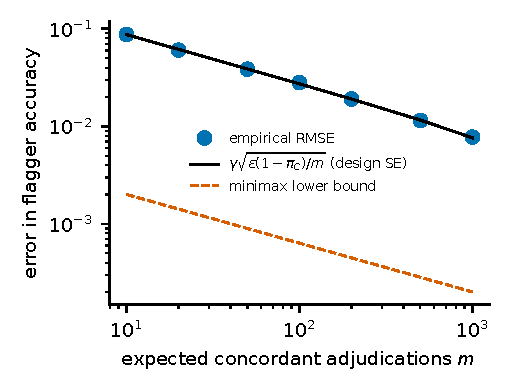
\includegraphics[width=0.55\linewidth]{figures/fig_rate.pdf}
\caption{Error of the two-phase estimate of the flagger's accuracy (Llama 3 70B, Scenario B with Mixtral 8x7B labels) against the expected number $m$ of concordant adjudications, with $\pi_\Dset=1$, over \reps{} replicates. The solid line is the design standard error (equation (3) of the paper); the dashed line is the minimax lower bound of Theorem~9 of the paper, evaluated at the observed $\gamma=\rateGamma$ and $\varepsilon=\rateEps$.}

\end{figure}

\end{document}
